Z~potřeb popsaných her vyplývají požadavky na~zařízení.
Tato zařízení lze rozdělit na~statická a~dynamická, podle toho, zda je~má hráč nosit všude s~sebou nebo s~nimi jen interaguje na~nehybném stanovišti.
V~obou dvou případech je~vhodné mít co~možná nejjednodušší metodu vytváření her.
Není tedy vhodné program pro každou hru psát v~samostatném projektu v~jazyce C.
Proto je~potřeba mít nějakou metodu, která umožní vytvářet hry v~nějakém jednodušším jazyce, např. v~Pythonu a~nebo JavaScriptu.

\section{Dynamická zařízení}
Dynamická zařízení jsou ta, která má~hráč nosit s~sebou.
Tato zařízení by~tedy měla být co~nejmenší a~nejlehčí, aby hráči nepřekáželo při pohybu.
Zároveň by~měla být co~nejlevnější, aby se~dala nasadit v~dostatečném množství.
Potřebuje také světelný výstup pro zobrazování herních stavů a~jednoduchý vstup pro ovládání. 

\section{Statická zařízení}
Statická zařízení jsou ta, u~nichž nepředpokládám, že~je bude hráč nosit s~sebou.
To ovšem neznamená, že~mohou být libovolně velká a~těžká, pořád je~potřeba, aby bylo snadné je~přesunout z~místa na~místo.
Stejně jako dynamická zařízení potřebují světelný výstup, aby bylo možno signalizovat herní stav a~reagovat na~hráče.
Také je~potřeba vstup, na~což většinou stačí obyčejná tlačítka.
Problém je~ale určit jaké a~kolik jich bude potřeba.
Některé hry vyžadují třeba jen jedno, ale takové, aby se~do něj dalo co~nejpohodlněji praštit v~běhu, protože je~zrovna cílem ke~stanovišti co~nejrychleji doběhnout jako třeba u~hry King of~the hill {viz: \ref{KOTH}}.
Jiná hra může vyžadovat tlačítek víc, ale už~není potřeba, aby byly tak velké, protože hráč při jejich používání nebude tak akční, ale bude třeba zadávat heslo, jako u~hry Špionská síť {viz: \ref{SpionskeSite}}.
Univerzálnější je~tedy nepoužívat tlačítka, ale nějaký systém, který se~dá softwarově přizpůsobit.
Příkladem může být dotyková plocha, která se~dá softwarově rozdělit na~různé oblasti sloužící jako tlačítka a~i~během hry se~tak dá~počet tlačítek měnit.
Další důležitou vlastností je~možnost komunikace s~ostatními zařízeními, která do~hry přináší novou možnost jak stanoviště propojit a~také pohodlnou metodu jak stanoviště nastavit přes telefon.
V~neposlední řadě je~vhodné mít zvukový výstup, který může být použit např. jako potvrzení zadaného hesla, nebo odezva na~prostý klik na~dotykovou plochu.

Aby ale bylo možné zařízení použít v~různých hrách, je~potřeba, aby bylo možné ho~přizpůsobit konkrétním potřebám.
Z~toho důvodu považuji za~vhodné k~základnímu zařízení moci připojit modul pro konkrétní herní mechaniky.
Z~toho tedy plyne diagram \ref{fig:diagram_zanoreni_0}.
\begin{figure}[h]
    \centering
    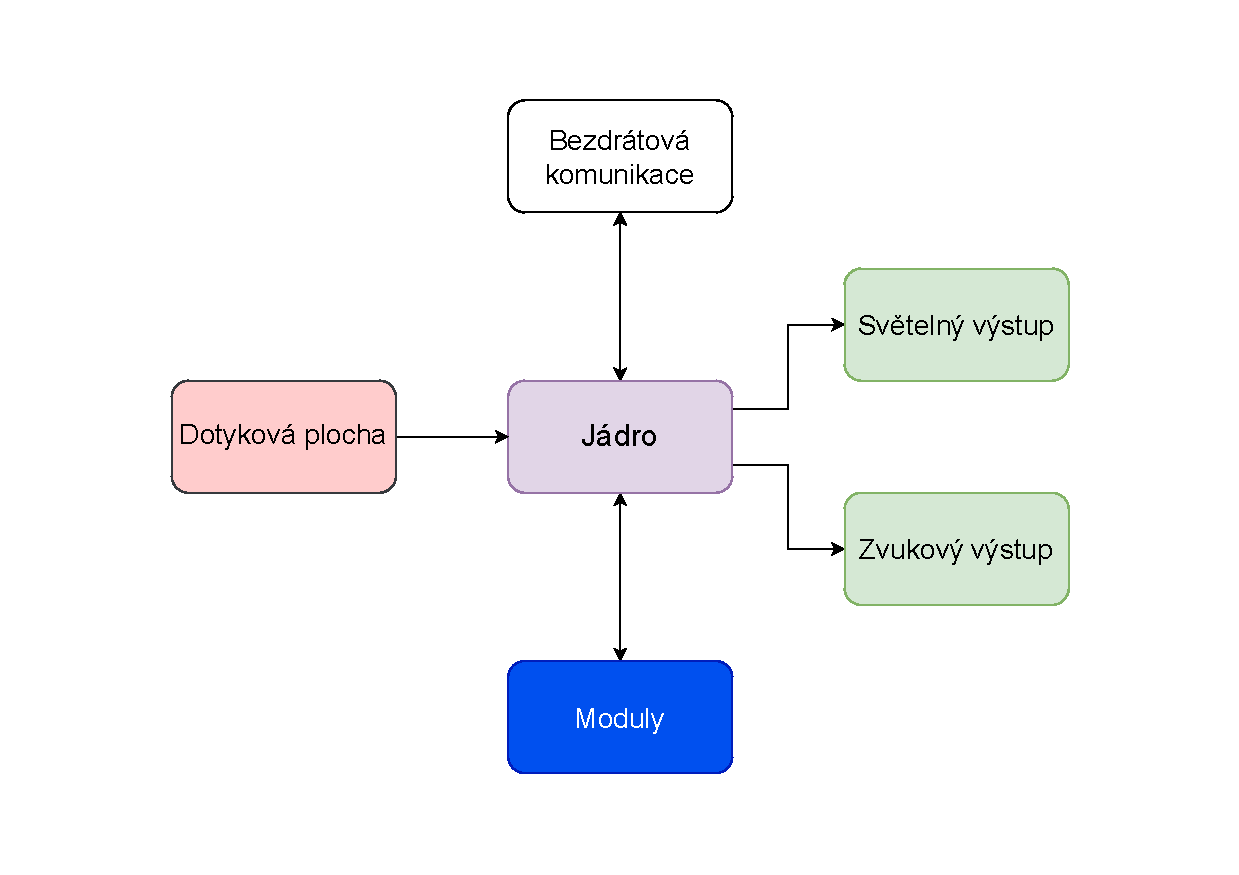
\includegraphics[width=\textwidth]{text/TeoretickyUvod/AplikaceHernichZarizeni/diagram/zanoreni_0.pdf}
    \caption{Úvodní blokové schéma zařízení}
    \label{fig:diagram_zanoreni_0}
\end{figure}

Co se~světelného výstupu týče, na~signalizaci různých stavů je~vhodné používat různé barvy světel.
% Jaký vzhled by~ale měl mít zdroj barevného světla na~podobném zařízení?
Jak je~vysvětleno v~následující části \ref{VyuzitiTelefonu}, není potřebné suplovat grafický display, za~tímto účelem se~dá použít propojení s~telefonem.
Informace, kterou zařízení bude často poskytovat, je~čas a~směr, např. čas do~konce kola nebo směr k~dalšímu úkolu.
Podobné informace se~dají elegantně zobrazit na~kruhu.
%Protože má~být stanoviště pohodlně čitelné z~blízky i~viditelné z~větší vzdálenosti, je~tedy otázkou, zda použít jen jeden kruh, tak aby byl dostatečně viditelný, nebo jich použít více. %%TODO: otázka co~s~totu otázkou?
Je vhodné zobrazování rozdělit na~dva režimy, čtení na~dálku a~čtení na~blízko.
Pro čtení na~blízko je~cílem přímá interakce se~zařízením, např. u~zadávání hesla.
Čtení na~dálku je~naopak určeno pro předávání informací hráči, když právě přímo neinteraguje se~stanovištěm, např. který tým má~zrovna povolený přístup do~zařízení.
Proto je~vhodné mít kruhů více, aby bylo možné zobrazovat tyto informace na~různých kruzích, které mohou navíc být svému účelu přizpůsobeny.
Jeden kruh tak může svítit jen jedním směrem, aby ho~hráč viděl celý najednou pro blízkou interakci, zatímco druhý kruh může svítit do~všech stran, aby byl vidět z~co nejvíce míst.

Potřeba propojení s~telefonem nám omezuje možnosti co~se týče typu bezdrátové komunikace, protože telefony jsou většinou vybaveny Bluetooth a~WiFi.
Také se~v~telefonech rozšiřuje NFC, to~je však pro tuto aplikaci z~důvodu krátkého dosahu nevhodné.

Posledním systémem, který je~třeba zmínit, je~zvukový výstup.
Protože většinou stačí jen jednoduchá zvuková odezva, není potřeba plnohodnotný zvukový systém.
Pro hry, které budou potřebovat přehrávat libovolnou nahrávku, může být použit samostatný zvukový modul, případně je~možnost nahrávku přehrát přes uživatelův telefon.
V~základním zařízení je~proto potřeba jen jednoduchý bzučák, například jako odezva na~kliknutí.
Můžeme tedy diagram upravit na~\ref{fig:diagram_zanoreni_1}.
\begin{figure}[h]
    \centering
    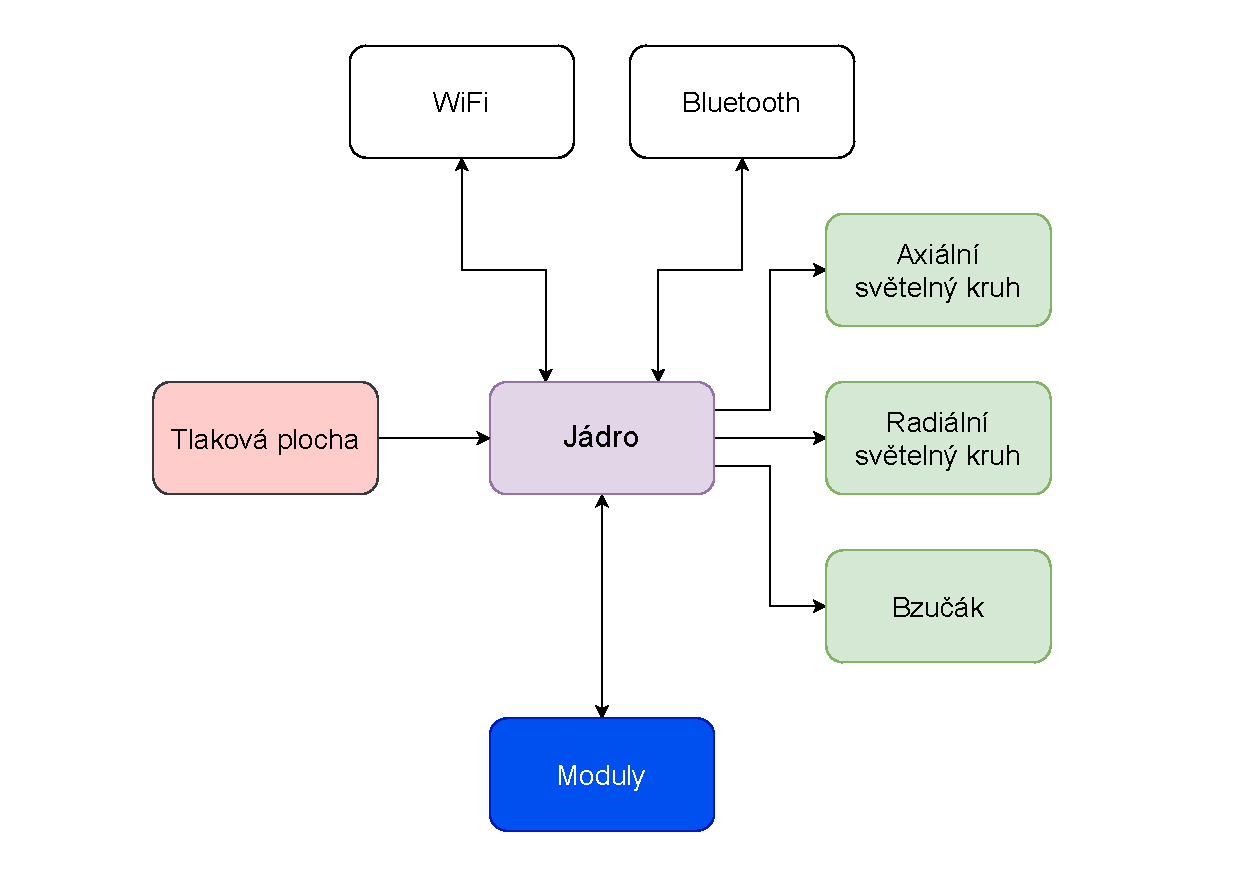
\includegraphics[width=\textwidth]{text/TeoretickyUvod/AplikaceHernichZarizeni/diagram/zanoreni_1.pdf}
    \caption{Základní blokové schéma zařízení}
    \label{fig:diagram_zanoreni_1}
\end{figure}

Celé zařízení by~také mělo být alespoň částečně voděodolné, aby se~dalo použít třeba i~za deště.

\section{Využití telefonu \label{VyuzitiTelefonu}}
Podstatný fakt je, že~prakticky všichni u~sebe dnes mají chytrý telefon, čehož mohu využít.
Nemá proto velký význam, aby statické nebo dynamické zařízení suplovalo funkce telefonu.
Např. grafický výstup typu display proto v~podobném zařízení není potřeba, a~v~tomto směru už~odvádí telefon naprosto dostatečnou práci.
Pokud by~tedy v~rámci hry bylo potřeba například předat hráči text nebo obrázek, může jej zařízení poslat uživateli na~telefon.
Telefon by~se tedy dal zařadit mezi dynamická zařízení.
Možnost propojení s~telefonem je~také velmi významná při nastavování hry.
Díky telefonu totiž zařízení nepotřebuje uživatelské rozhraní přizpůsobené k~nastavování, ale prostě se~vše nastaví z~telefonu.

Někdy by~se mohlo zdát, že~herní stanoviště vlastně ani není potřeba a~stačila by~mobilní aplikace.
Ale přestože je~mobil ve~hrách dobře využitelný, jsou aplikace, na~které jednoduše vhodný není.
Pokud má~hráč například ze~stanoviště získat fyzický objekt, mobil neposlouží.
Pro hráče ani organizátory také nemusí být zrovna komfortní před hrou zařizovat, aby měli všichni nainstalovaný správný software.
% Telefon také není například na~stanovišti v~lese dobře viditelný.
V~neposlední řadě jde také o~jistý "cool efekt", který běžné zařízení jako mobil nebo třeba tablet neposkytne. %%TODO: tohle chce nějak přeformulovat

